\documentclass{standalone}
\usepackage{tikz}

\begin{document}

\begin{tikzpicture}
    % Define a variable for the circle radius
    \def\circleradius{0.2cm}
    \def\offset{0.3cm}
    \def\distance{2cm}
    \def\onenode{0.7cm}

     % Define light grey color
     \colorlet{mygrey}{gray}

    % X-axis: Draw lines between circles
    \draw[-, color=mygrey, thick]  (-0.2cm,0) -- (1*\distance - \onenode-\circleradius,0);
    \draw[-, color=mygrey, thick]  (1*\distance - \onenode+\circleradius,0) -- (2*\distance - \onenode-\circleradius,0);
    \draw[-, color=mygrey, thick]  (2*\distance - \onenode+\circleradius,0) -- (3*\distance - \onenode-\circleradius,0);
    \draw[->,  color=mygrey, >=stealth, thick] (3*\distance - \onenode+\circleradius,0) -- (4*\distance - \onenode,0) node[right] {loops};

    % Y-axis: Draw lines between circles
    \draw[-, color=mygrey, thick]  (0,0.2cm) -- (0,-1*\distance + \onenode + \circleradius);
    \draw[-, color=mygrey, thick]  (0,-1*\distance + \onenode-\circleradius) -- (0,-2*\distance + \onenode+\circleradius);
    \draw[-, color=mygrey, thick]  (0,-2*\distance + \onenode-\circleradius) -- (0,-3*\distance + \onenode+\circleradius);
    \draw[->, color=mygrey, >=stealth, thick] (0,-3*\distance + \onenode-\circleradius) -- (0,-4*\distance + \onenode) node[below] {legs};

    % Place smaller circled labels on the x-axis
    \node[circle, draw=black, minimum size=\circleradius*2, inner sep=1pt, color=mygrey, thick] at (1*\distance - \onenode, 0) {1};
    \node[circle, draw=black, minimum size=\circleradius*2, inner sep=1pt, color=mygrey, thick] at (2*\distance - \onenode, 0) {2};
    \node[circle, draw=black, minimum size=\circleradius*2, inner sep=1pt, color=mygrey, thick] at (3*\distance - \onenode, 0) {3};

    % Place smaller circled labels on the negative y-axis
    \node[circle, draw=black, minimum size=\circleradius*2, inner sep=1pt, color=mygrey, thick] at (0,-1*\distance + \onenode) {3};
    \node[circle, draw=black, minimum size=\circleradius*2, inner sep=1pt, color=mygrey, thick] at (0,-2*\distance + \onenode) {4};
    \node[circle, draw=black, minimum size=\circleradius*2 ,inner sep=1pt, color=mygrey, thick] at (0,-3*\distance + \onenode) {5};

   \node at (1*\distance - 1.3*\onenode, -1*\distance + 1*\onenode) {\includegraphics[scale=0.044]{1loop_3.eps}};
   \node at (2*\distance - 1.3*\onenode, -1*\distance + 1*\onenode) {\includegraphics[scale=0.044]{2loop_3.eps}};
   \node at (3*\distance - 1.3*\onenode, -1*\distance + 1*\onenode) {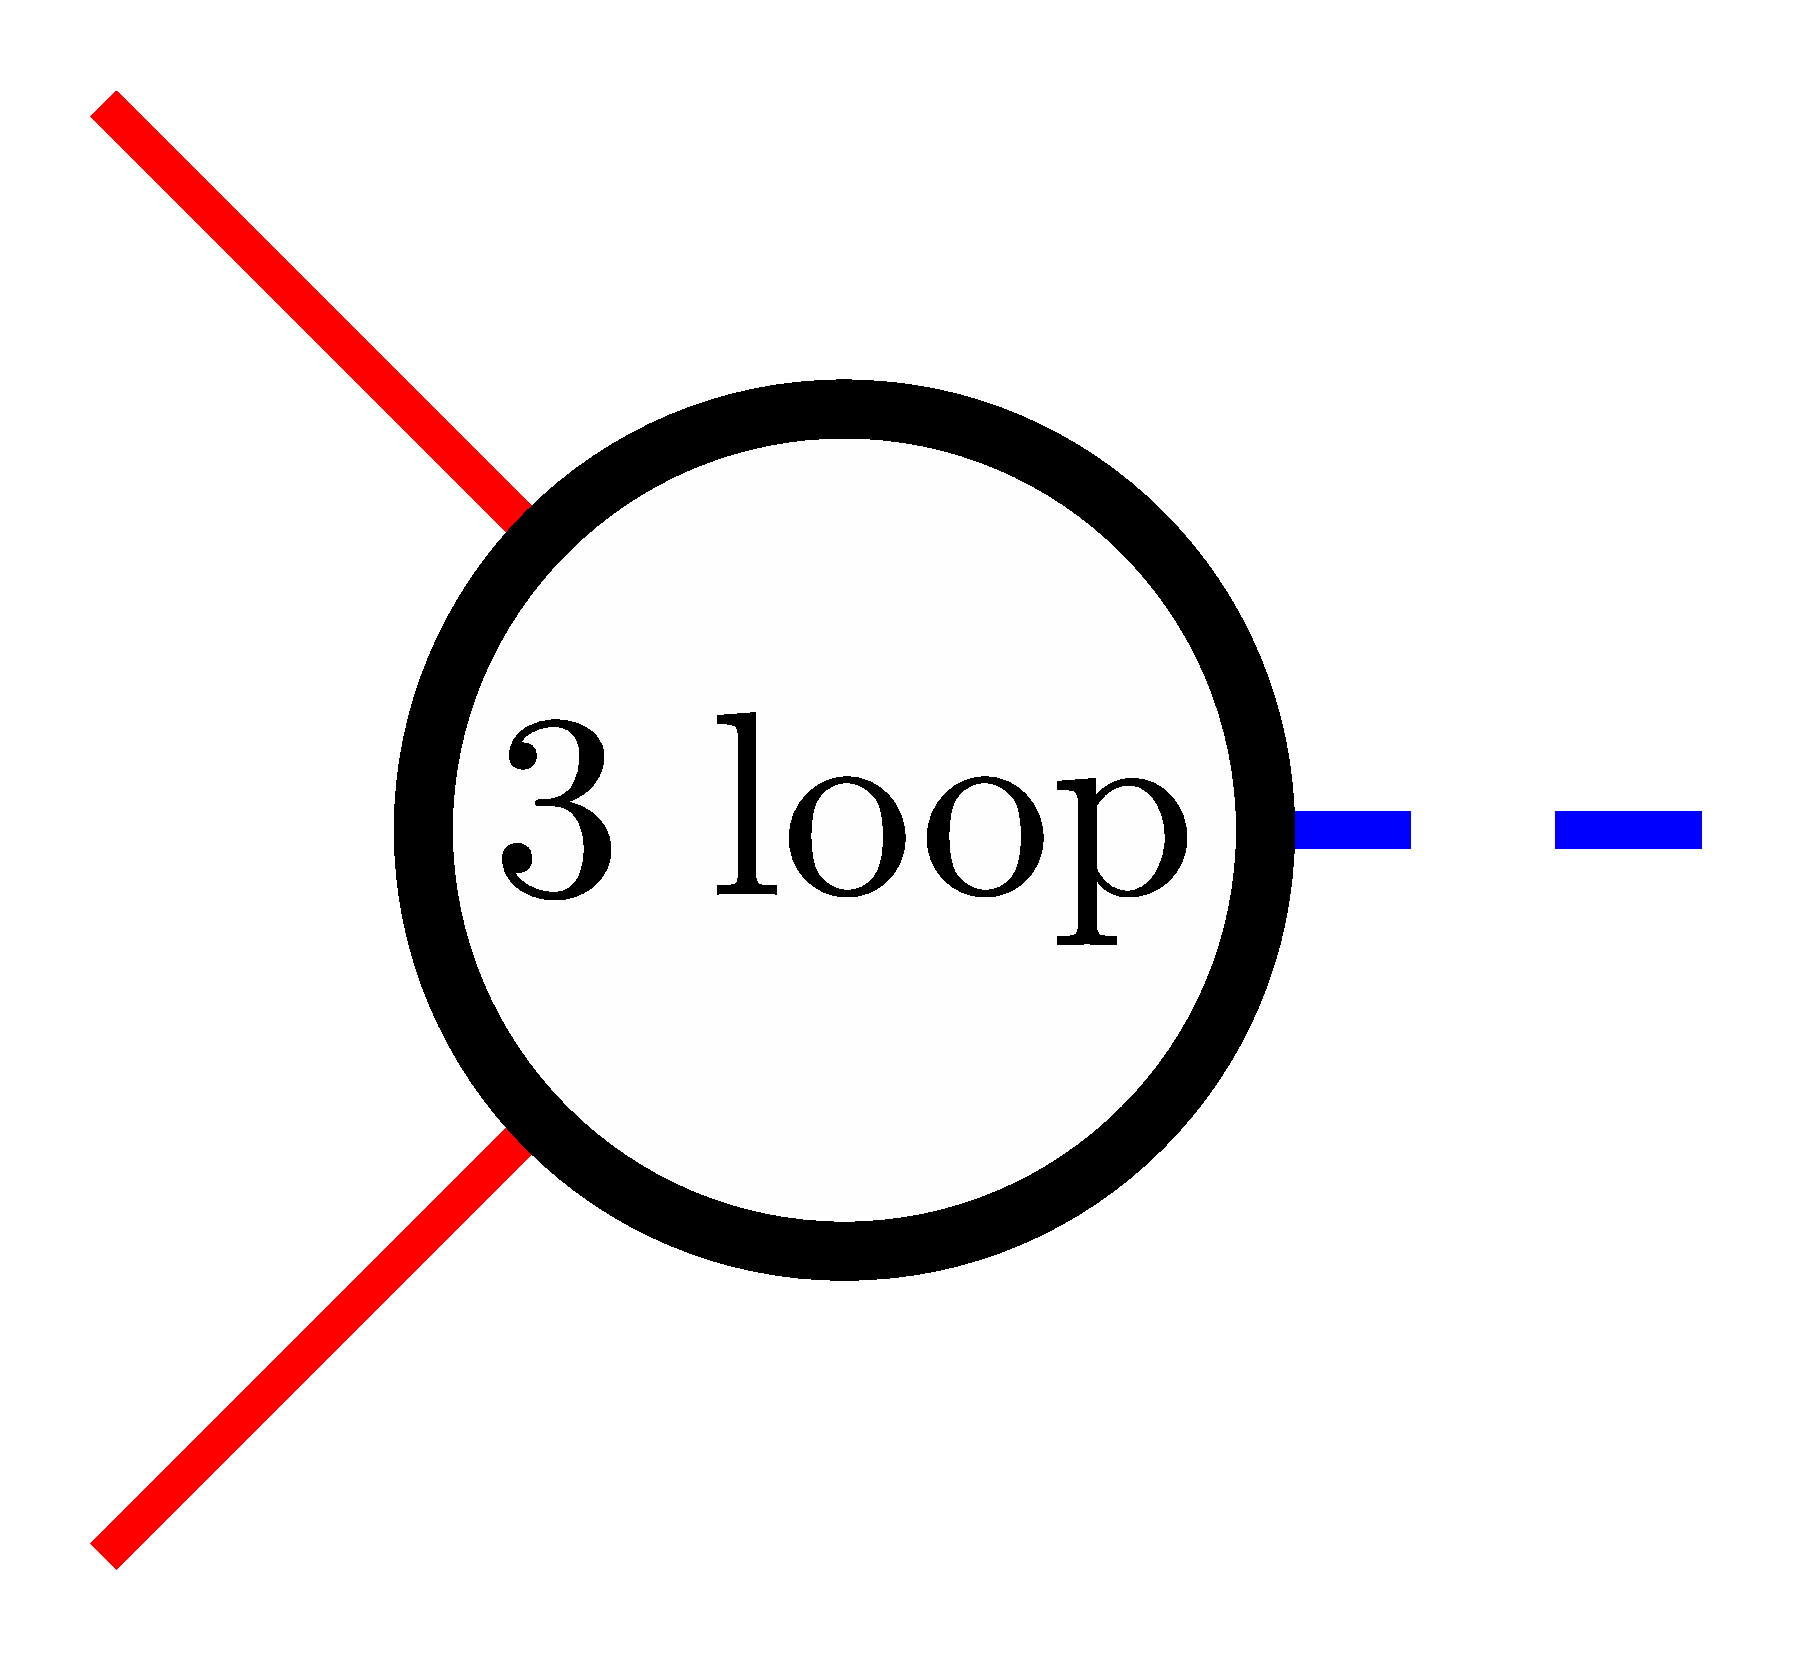
\includegraphics[scale=0.044]{3loop_3.eps}};
   \node at (1*\distance - 1.3*\onenode, -2*\distance + 1*\onenode) {\includegraphics[scale=0.044]{1loop_4.eps}};
   \node at (2*\distance - 1.3*\onenode, -2*\distance + 1*\onenode) {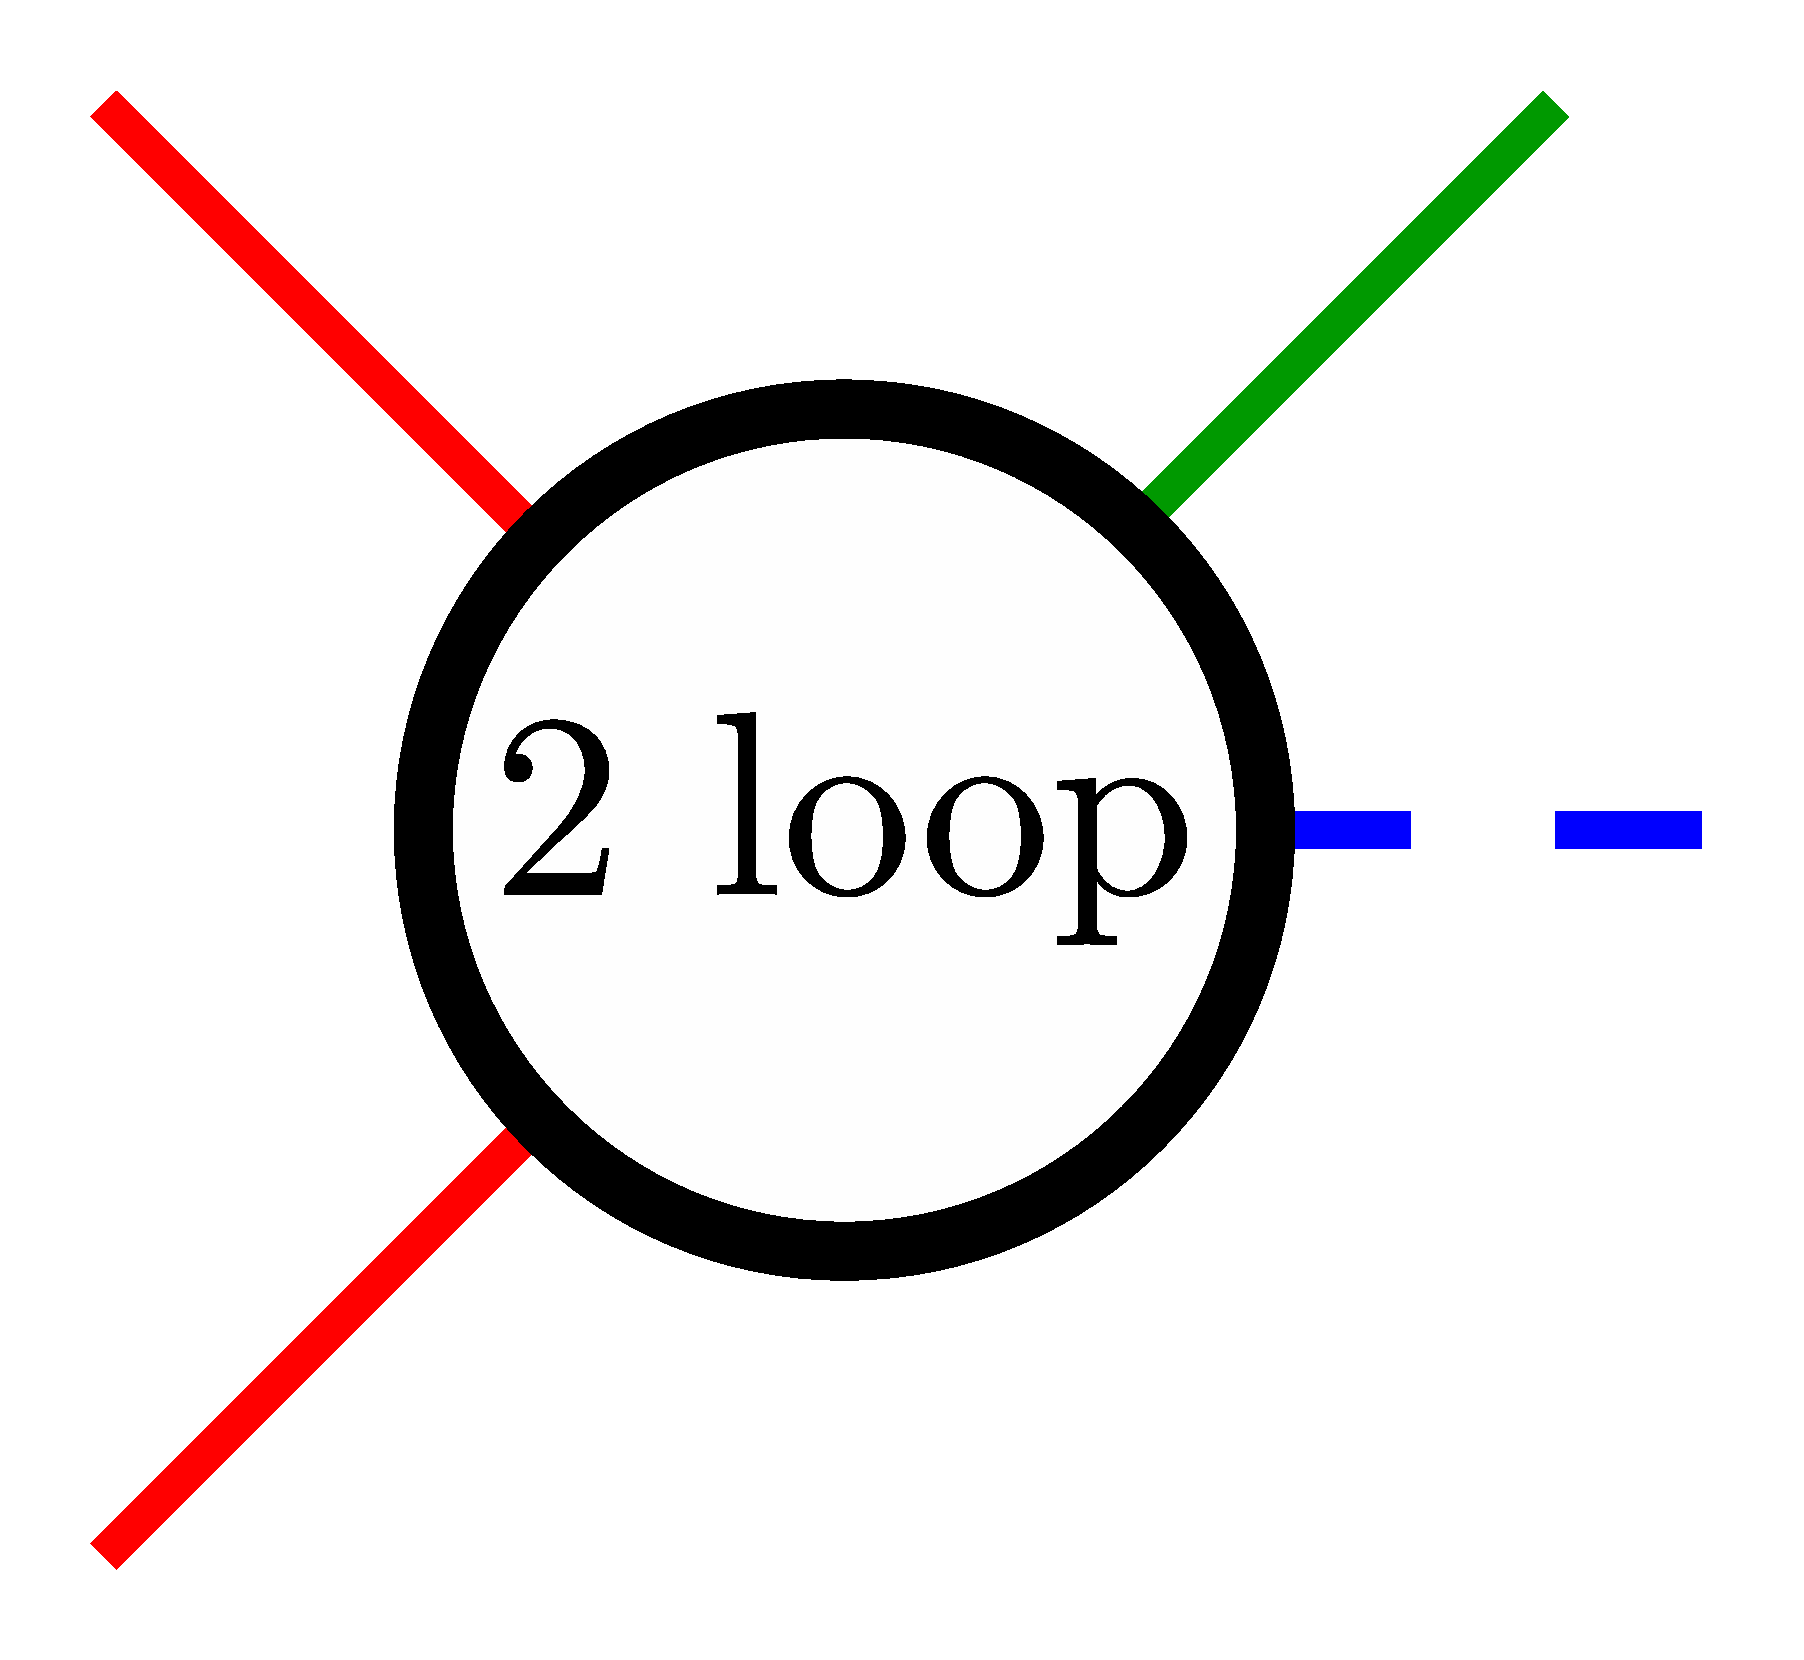
\includegraphics[scale=0.044]{2loop_4.eps}};
   \node at (1*\distance - 1.3*\onenode, -3*\distance + 1*\onenode) {\includegraphics[scale=0.044]{1loop_5.eps}};

   % Draw diagonal lines connecting labels without crossing circle boundaries
   \draw[-, color=mygrey] (\offset,-2*\distance + \onenode+1.5*\offset) -- (2*\distance - \onenode - 1.5*\offset, -\offset);
   \draw[-, color=mygrey] (\offset,-3*\distance + \onenode+1.5*\offset) -- (3*\distance - \onenode - 1.5*\offset, -\offset);
   \draw[-, color=mygrey] (\offset,-4*\distance + \onenode+1.5*\offset) -- (4*\distance - \onenode - 1.5*\offset, -\offset);

   \node at (1*\distance - \onenode + 2.5*\offset, - \offset) {LO};
   \node at (2*\distance - \onenode + 2.5*\offset, - \offset) {NLO};
   \node at (3*\distance - \onenode + 2.5*\offset, - \offset) {NNLO};


\end{tikzpicture}

\end{document}